\documentclass[12pt]{article}
\usepackage[utf8]{inputenc}
\usepackage[super]{natbib}
\usepackage{indentfirst}
\usepackage{graphicx}
\usepackage{fancyhdr}
\usepackage{url}

\pagestyle{fancy}
\fancyhf{}
\lhead{Communication and social media}
\cfoot{\thepage}

\title{\vspace{-3em} Communication models and cultural influence. Social media in contemporary world}
\author{Karol Latos\\Macrofaculty group 2}
\date{}

\begin{document}

\maketitle

\section{What is communication?} \noindent
Communication is...

\begin{quotation}
...the act of conveying intended meanings
from one entity or group to another through
the use of mutually understood signs and
semiotic rules.
\end{quotation}

\textit{But what does that mean? \vspace{+0.5em}} \par

Communication is any process of transmitting information from one agent to another. This way, we perceive the act of communicating as detached from strictly social realm. The conversation between humans is a particular example of communication, similarly to the active connection between two servers or the exchange of calls made by blue whales. Astonishingly, the latter serves as:

\begin{enumerate}
\setlength\itemsep{0.3em}
\item{maintenance of inter-individual distance;}
\item{species and individual recognition;}
\item{contextual information transmission (e.g. feeding, alarm, courtship);}
\item{maintenance of social organization (e.g. contact calls between females and males);}
\item{location of topographic features;}
\item{location of prey resources.\cite{whales}}
\end{enumerate} \par

This gives us a glimpse into the natural need for communication and its usefulness. If the world is composed of information, then communication is the process by which the reality comes to life.

\section{Basic models of communication}
The act of communication can be abstracted out and modeled in various ways. This concept alone is a broad section of communication theory --- a field of science on the frontier between mathematics, information theory, psychology, sociology, anthropology and semiotics. Selected models are briefly presented.

\subsection{Linear Model}
The Linear Model, constructed by Claude Shannon in 1948 and popularized by Warren Weaver in 1949, is the first model of communication, called the \textit{mother of all models}\cite{mothermodel}.

\begin{figure}[htp]
    \centering
    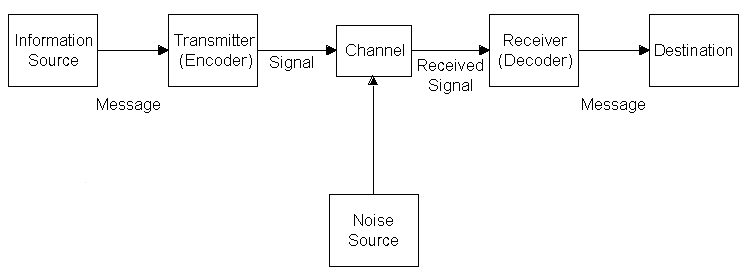
\includegraphics[width=\textwidth]{lin.png}
    \caption{Shannon-Weaver model of communication (1949)}
    \label{lin}
\end{figure}

It works in one direction only: a sender encodes a message and sends it through a channel for a receiver to decode.

\subsection{Interactional Model}
In comparison, the Interactional Model (or Interactive Model) of communication is bidirectional, i.e. agents send and receive messages in a cooperative way, as they continuously encode and decode information. \pagebreak \par
This model was proposed by Wilber Schramm in 1954 and it emphasizes two things on top of the Shannon-Weaver model:

\begin{enumerate}
    \item The communication ought to be continuous in time by \textbf{alternating the roles} of sender and receiver.
    \item Coding and decoding are the \textbf{two essential processes} of an effective communication.
\end{enumerate}

\begin{figure}[htp]
    \centering
    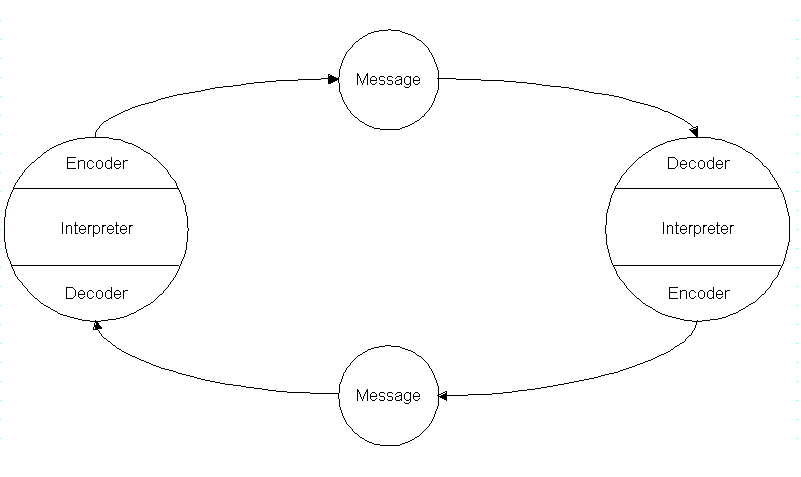
\includegraphics[width=\textwidth]{int.png}
    \caption{Schramm's model of communication (1954)}
    \label{int}
\end{figure}

Communication is then described as a process in which participants alternate between the positions of senders and receivers (Fig \ref{int}).

\subsection{Transactional Model}

As humanity progressed into the era of Internet and interconnectedness on a global scale, a new model emerged; one that described the \textit{fluid} and \textit{contextual} nature of human communication. Contrued by Dean C. Barnlund in 1970\cite{barnlund}, the transactional model depicted communication as a process in which communicators create their own contribution to social, relational, and cultural contexts. In contrary to previous models, participants are not labeled as senders and receivers, but rather communicators, incarnating both roles at the same time.

\begin{figure}[htp]
    \centering
    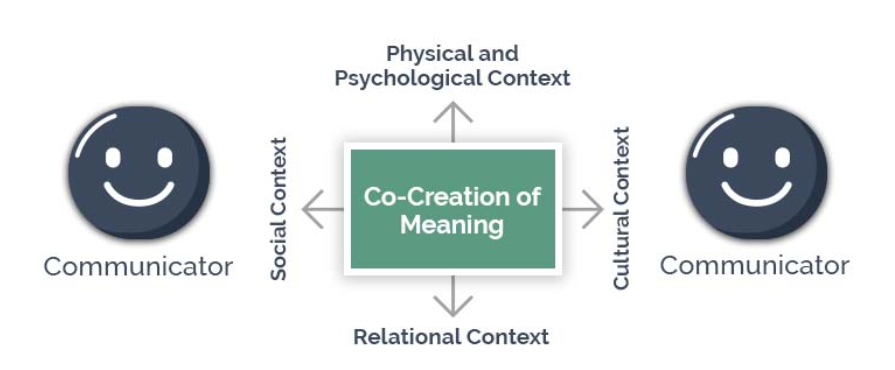
\includegraphics[width=\textwidth]{tra.png}
    \caption{Barnlund model of communication (1970, simplified\cite{transactional})}
    \label{tra}
\end{figure}


Main implications of the transactional model:
\begin{enumerate}

\item{Communication is an \textbf{enduring and altering}, rather than one time process. Individuals and the environment can change as per the circumstances.}

\item{Each element exists concerning \textbf{all other elements} and all individuals are \textbf{interdependent}.}

\item{Every communicator reacts accordingly to their \textbf{cultural beliefs}, \textbf{personal experiences}, \textbf{attitudes}, and \textbf{social norms}.}

\item{People can \textbf{exchange} their views and ideas.}
\end{enumerate}

\section{How does the culture influence communication?}
Focusing on the cultural aspect of human communication, there is a lot to say; we're not the only species to exchange signals or encoded messages, but we're the only one to use abstract language for that purpose. The ever-going struggle to find the right relationship between the signifier and the signified is heavily influenced by the culture we're brought up in. Lacan believed that we cannot ever close the gap between the words and the meanings we want to convey, and that everything inexpressible (or \textit{suppressed}) forms the unconscious\cite{lacan}. That implies that our psychological context is molded by the set of meanings that we understand (like the concept of a tree), and the set of words and symbols that we use to describe those meanings (like the word \textit{tree}). Since these sets will differ largely between cultures, one can argue that there exist profound cognitive differences between nations, tribes or civilizations. \par
Another important point is the existence of social norms defined culturally. In cultures, where socializing plays an important part, a foreign businessman may be invited to a sauna (Finland) or karaoke bar (Japan) a day before work meeting; something unusual to some Western countries (individualism, separation of personal and work life). \par
One specific example may be the attitude towards presentations of projects or business ideas. Presenters from United States will talk about future prospects, predicted sales and market niches, while presenters from China or India will focus on previous accomplishments, established credibility and sale details. This dissonance between future- and past-oriented perspectives is one of many cultural factors influencing the successfulness of communication.

\section{How do social media create thr reality of our everyday life?}
The role of Internet in today's world is unprecedented. From social point of view there is no doubt that social media, i.e. web platforms for sharing, creating and viewing content by users, influenced the state of our lives. Some of these effect are positive, like the increased sense of connectedness with online or real communities; more effective marketing for corporations, charities and political parties; immediate communication with friends or work associates; and generating new, creative content with little budget or amateur setup (like Youtube). Moreover, many businesses use social media for consumer-friendly marketing, discounts and feedback about the product. However, the effects of social media go both ways: among other things, a rise in depression rate, loneliness and harassment has been observed, especially among adolescent users of Instagram and Snapchat, where the impact on mental health has the highest net negative values (Fig \ref{socmedChart}).

\begin{figure}[htp]
    \centering
    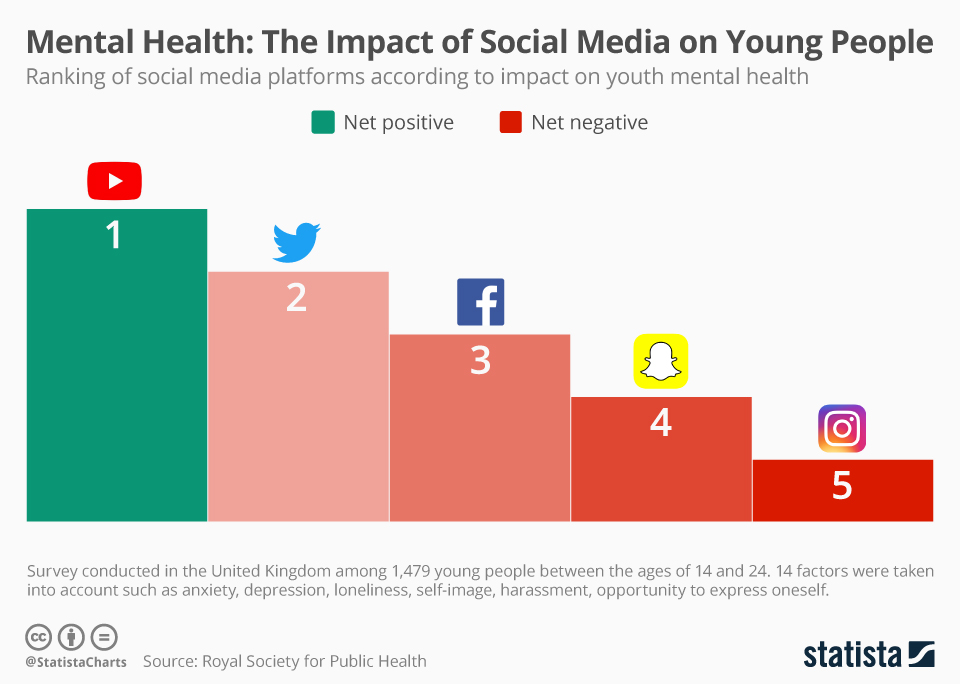
\includegraphics[width=0.9\textwidth]{socmed.jpeg}
    \caption{The impact of social media on adolescents aged 14-24\cite{socmed}}
    \label{socmedChart}
\end{figure}

Additionally, not every online marketing strategy is ethical. One example would be the Facebook---Cambridge Analytica data scandal, where the personal information of millions of Facebook users was used for targeting political advertisements. This poses a question about how powerful social media really are --- are they influential enough to change the result of an election? --- and how should we act in the light of new problems concerning data mining, privacy and authorship. \par
The cyber-world of social media is still an uncharted territory and the number of ethical difficulties that lie ahead is most likely astronomical. Social media mold the fabric of our societies and ourselves, but they are undeniably an advancement on the social scale of humanity. And like with many other advancements, we accept them with their positive and negative effects, trying our best to mitigate the latter.

\begin{thebibliography}{4}

\bibitem{whales}
Richardson, W.J.; Green, C.R., Jr.; Malme, C.I.; Thomson, D.H. (1995). ``Marine mammals and noise". Academic Press. San Diego, CA.

\bibitem{mothermodel}
Hollnagel, E.; Woods, D.D. (2005). ``Joint Cognitive Systems: Foundations of Cognitive Systems Engineering''. Boca Raton, FL. Taylor \& Francis.
ISBN 978-0-8493-2821-3.

\bibitem{barnlund}
Barnlund, D.C. (2008). ``A transactional model of communication''. In. Mortensen C.D. (Eds.), ``Communication theory'' (2nd ed., pp 47-57). New Brunswick, NJ.

\bibitem{transactional}
\small\url{https://calltutors.com/blog/transactional-model-of-communication/}
(Accessed 16.05.2020)

\bibitem{lacan}
Lacan, J (1964). ``The Seminar. Book XI. The Four Fundamental Concepts of Psychoanalysis''. Trans. Alan Sheridan. London: Hogarth Press and Institute of Psycho-Analysis, 1977, pp 126

\bibitem{socmed}
Royal Society for Public Health (2017) ``Status of Mind. Social media and young people's mental health and wellbeing''

\end{thebibliography}

\end{document}
